\documentclass[aspectratio=169,11pt]{beamer}

\usepackage[T1]{fontenc}
\usepackage{lmodern}
\usepackage{xcolor}
\usepackage{tikz}
\usepackage{booktabs}
\usepackage{array}
\usepackage{listings}
\usepackage{textcomp}

\definecolor{navy}{HTML}{0A2540}
\definecolor{orange}{HTML}{D97706}
\definecolor{green}{HTML}{15803D}
\definecolor{grey}{HTML}{6B7280}
\definecolor{lightgrey}{HTML}{E5E7EB}
\definecolor{red}{HTML}{B91C1C}
\definecolor{codebg}{HTML}{F8FAFC}
\definecolor{lightorange}{HTML}{FED7AA}
\definecolor{lightnavy}{HTML}{DBEAFE}
\definecolor{lightred}{HTML}{FECACA}

\usecolortheme[named=navy]{structure}
\setbeamertemplate{navigation symbols}{}
\setbeamercolor{frametitle}{fg=navy}
\setbeamerfont{frametitle}{series=\bfseries,size=\Large}
\setbeamertemplate{footline}{%
  \hbox{\hspace{0.9em}\color{grey}\tiny exp27 \textperiodcentered\
    1B vs 1.5B cross-model check \textperiodcentered\
    MarinFold\hfill\insertframenumber{} / \inserttotalframenumber\hspace{0.9em}}\vspace{0.3em}}
\setbeamertemplate{frametitle}{%
  \vspace*{0.4em}\hspace*{0.6em}\insertframetitle\par
  \vspace*{-0.2em}\hspace*{0.6em}\textcolor{orange}{\rule{0.93\paperwidth}{1.2pt}}\vspace*{-0.4em}
}

\lstdefinestyle{code}{
  basicstyle=\ttfamily\small\color{navy},
  backgroundcolor=\color{codebg},
  frame=single, framerule=0.4pt, rulecolor=\color{navy},
  numbers=none, breaklines=false, showstringspaces=false,
  xleftmargin=0.6em, xrightmargin=0.6em, aboveskip=0.4em, belowskip=0.4em,
}
\newcommand{\code}[1]{\texttt{\small\color{navy}#1}}
\newcommand{\codeS}[1]{\texttt{\scriptsize\color{navy}#1}}

\begin{document}

% --- Slide 1: title ---
\begin{frame}[plain]
  \begin{center}
    \vspace{0.6cm}
    {\Huge\bfseries\color{navy}Does the 1B algorithm transfer to 1.5B?}\\[0.4cm]
    {\Large\color{navy}\codeS{iter\_R4\_grow\_on\_sampled\_uniform\_M5}}\\
    {\Large\color{navy}re-run on the new \codeS{1.5B} (step-49999)}\\[0.7cm]
    {\Large\color{red}\bfseries Short answer: no.}\\[0.4cm]
    {\large\color{navy}\textbf{1B}: +42.81\% over baseline\\[0.2em]
     \textbf{1.5B}: only +9.04\% — and stage A alone is \emph{worse} than baseline.}\\[1.2cm]
    {\small\color{grey}\ttfamily Same 10 train proteins \textperiodcentered\
      same hyperparameters \textperiodcentered\ A100 40\,GB bf16}
  \end{center}
\end{frame}

% --- Slide 2: setup ---
\begin{frame}{Setup}
  \begin{itemize}
    \setlength\itemsep{0.4em}
    \item Rebased \code{exp/27-improved-inference-algorithm} onto main \textrightarrow{}
          \code{MODELS.yaml} now lists \code{1.5B}\\
          (\codeS{buckets/open-athena/MarinFold/.../protein-contacts-1\_5b-distance-masked-70f8f5/step-49999}).
    \item Architecture: \textbf{24 hidden layers} (vs 1B's 16), hidden 2048,
          \textbf{8 KV heads / 32 query heads} (GQA), intermediate 8192.
          $\sim$1.5$\times$ the parameters of 1B.
    \item Checkpoint name \codeS{step-49999} suggests \textbf{undertrained}
          relative to the 1B production checkpoint.
    \item Algorithm and knobs held \textbf{exactly identical to the 1B
          headline}: \code{sampled\_uniform\_M5\_union} prior + \code{iter\_R4\_grow}
          on top, \code{range\_strategy=uniform},
          \code{kc=[0.5, 1, 1.5, 2.5]}, \code{min\_contact\_prob=0.1},
          standard expected-distance readout, no sharpening.
    \item Same 10-protein train set, output to \codeS{outputs\_1.5b/} so 1B
          snapshots are preserved.
  \end{itemize}
\end{frame}

% --- Slide 3: headline table ---
\begin{frame}{Headline numbers}
  \begin{center}\small
    \begin{tabular}{lrrr@{\hspace{1.5em}}l}
      \toprule
      run & mean LDDT & median & wall (s) & lift\\
      \midrule
      1B baseline (naive)            & 0.2496 & 0.2500 & 1387 & --- \\
      \textbf{1B combined}           & \textbf{0.3564} & 0.3665 & 3155 & \textcolor{green}{\textbf{+42.81\%}}\\
      \addlinespace
      1.5B baseline (naive)          & 0.2627 & 0.2577 & 1866 & --- \\
      1.5B stage A only              & 0.2038 & 0.2126 & 3472 & \textcolor{red}{\textbf{$-$22.42\%}} \\
      \textbf{1.5B combined}         & \textbf{0.2864} & 0.2665 & 4230 & \textcolor{orange}{\textbf{+9.04\%}}\\
      \bottomrule
    \end{tabular}
  \end{center}
  \vspace{0.2em}
  {\scriptsize\color{grey}stage A = \codeS{sampled\_uniform\_M5\_union};\ \
    combined = \codeS{iter\_R4\_grow\_on\_sampled\_uniform\_M5}.}
  \vspace{0.6em}
  \begin{itemize}
    \setlength\itemsep{0.2em}
    \item 1.5B \emph{baseline} is only modestly better than 1B (+5\%).
    \item 1.5B with the algorithm gives \textbf{0.2864} — worse in absolute
          terms than the 1B combined result (0.3564) and the lift over
          its own baseline drops from \textbf{+42.81\%} \textrightarrow{}
          \textbf{+9.04\%}.
    \item \textbf{Stage A alone (sampled\_uniform\_M5\_union) is below the
          1.5B baseline} — sampled-uniform contacts hurt the 1.5B model.
  \end{itemize}
\end{frame}

% --- Slide 4: per-protein ---
\begin{frame}{Per-protein lift (combined vs same-model baseline)}
  \begin{center}
    \begin{tabular}{lrrrrrr}
      \toprule
      stem & L & 1B base & 1B combined & 1B lift & 1.5B combined & 1.5B lift\\
      \midrule
      8eb9 &  95 & 0.1510 & 0.3071 & +128.8\% & 0.2665 & \textcolor{green}{+78.1\%}\\
      7y5j & 102 & 0.4485 & 0.5136 & +14.6\%  & 0.5645 & \textcolor{green}{+6.0\%}\\
      7ykm & 105 & 0.3317 & 0.4639 & +39.9\%  & 0.4010 & \textcolor{green}{+28.4\%}\\
      7ur2 & 195 & 0.2633 & 0.3665 & +39.2\%  & 0.3090 & \textcolor{green}{+19.9\%}\\
      8baq & 208 & 0.1872 & 0.2567 & +37.1\%  & 0.2425 & \textcolor{green}{+30.8\%}\\
      8cba & 214 & 0.2045 & 0.3028 & +48.1\%  & 0.2772 & \textcolor{green}{+35.0\%}\\
      7zs2 & 316 & 0.2500 & 0.3778 & +51.1\%  & 0.2086 & \textcolor{red}{\textbf{$-$25.7\%}}\\
      7xz3 & 325 & 0.1913 & 0.2727 & +42.6\%  & 0.2146 & \textcolor{green}{+6.7\%}\\
      7ylr & 330 & 0.2673 & 0.3991 & +49.3\%  & 0.2140 & \textcolor{red}{\textbf{$-$30.3\%}}\\
      7uk8 & 394 & 0.2010 & 0.2657 & +32.2\%  & 0.1661 & \textcolor{red}{\textbf{$-$14.6\%}}\\
      \bottomrule
    \end{tabular}
  \end{center}
  \vspace{0.4em}
  {\small\color{navy}\textbf{Pattern: the 3 regressions on 1.5B are the
    3 longest proteins} (L=316, 330, 394). Small / mid proteins still
    benefit but with smaller gains than on 1B. The mean is dragged down
    by the long-protein failures.}
\end{frame}

% --- Slide 5: per-protein chart ---
\begin{frame}{Visual: 1B combined (orange) vs 1.5B combined (red)}
  \begin{center}
    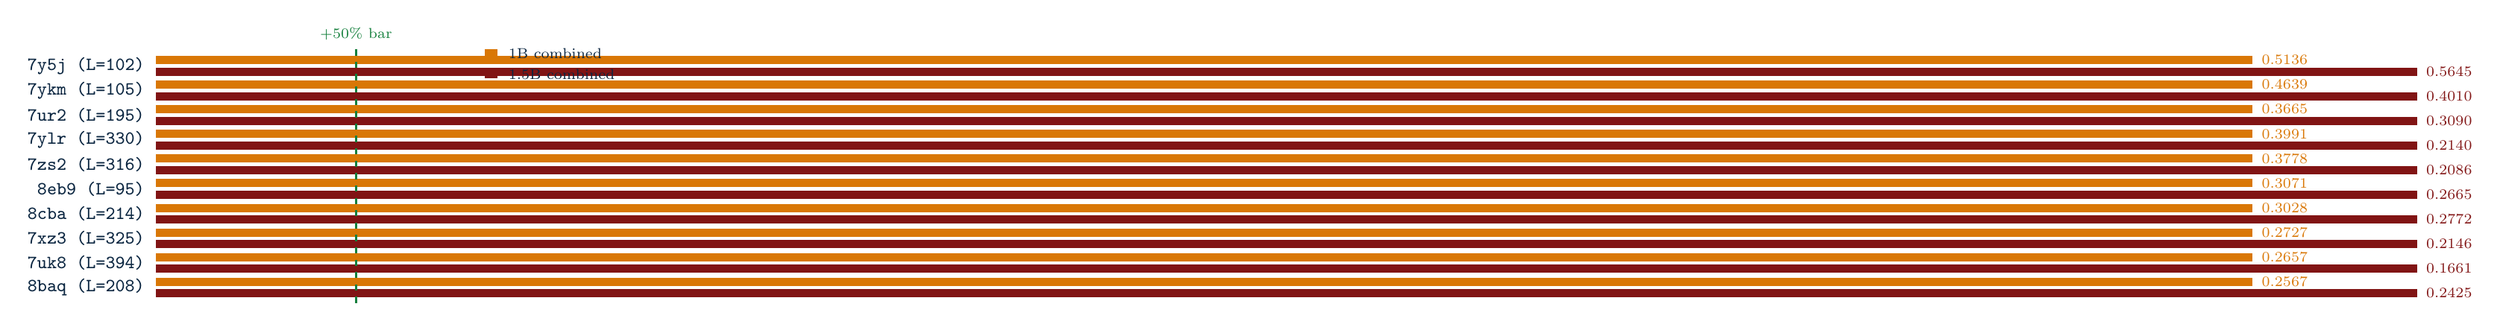
\begin{tikzpicture}[scale=0.70]
      \foreach[count=\i from 0] \name/\Len/\fone/\ffive in {%
        7y5j/102/0.5136/0.5645,
        7ykm/105/0.4639/0.4010,
        7ur2/195/0.3665/0.3090,
        7ylr/330/0.3991/0.2140,
        7zs2/316/0.3778/0.2086,
        8eb9/95/0.3071/0.2665,
        8cba/214/0.3028/0.2772,
        7xz3/325/0.2727/0.2146,
        7uk8/394/0.2657/0.1661,
        8baq/208/0.2567/0.2425
        } {
        \pgfmathsetmacro\yp{-\i * 0.60}
        \node[anchor=east, text=navy, font=\small\ttfamily]
          at (-0.1, \yp) {\name\ (L=\Len)};
        \pgfmathsetmacro\wf1{\fone * 13}
        \pgfmathsetmacro\wf5{\ffive * 13}
        \fill[orange] (0, \yp + 0.04) rectangle ++(\wf1, 0.20);
        \fill[red!70!black] (0, \yp - 0.24) rectangle ++(\wf5, 0.20);
        \node[anchor=west, font=\scriptsize, text=orange]
          at (\wf1 + 0.05, \yp + 0.14) {\fone};
        \node[anchor=west, font=\scriptsize, text=red!70!black]
          at (\wf5 + 0.05, \yp - 0.14) {\ffive};
      }
      % +50% bar
      \draw[green, line width=1.0pt, dashed]
        (0.3744*13, 0.4) -- (0.3744*13, -5.9);
      \node[anchor=south, font=\scriptsize, text=green]
        at (0.3744*13, 0.45) {+50\% bar};
      % Legend
      \fill[orange] (8.0, 0.2) rectangle ++(0.3, 0.2);
      \node[right, font=\scriptsize, text=navy]
        at (8.4, 0.3) {1B combined};
      \fill[red!70!black] (8.0, -0.3) rectangle ++(0.3, 0.2);
      \node[right, font=\scriptsize, text=navy]
        at (8.4, -0.2) {1.5B combined};
    \end{tikzpicture}
  \end{center}
  \vspace{0.1em}
  {\footnotesize\color{navy}Long proteins on 1.5B (7ylr, 7zs2, 7uk8 — bottom)
    drop dramatically. 7y5j and 8cba are the only proteins where 1.5B beats
    1B.}
\end{frame}

% --- Slide 6: stage A diagnostic ---
\begin{frame}{Where it breaks: stage A makes things worse}
  \begin{center}
    \begin{tabular}{lrrr}
      \toprule
       & 1B & 1.5B & delta\\
      \midrule
      baseline (naive readout)       & 0.2496 & 0.2627 & +0.013 \\
      stage A only (sampled\_uniform\_M5\_union) & \textbf{0.3142} & \textbf{0.2038} & \textbf{$-$0.111} \\
      stage A lift vs baseline       & \textcolor{green}{+25.9\%} & \textcolor{red}{\textbf{$-$22.4\%}} & \\
      \midrule
      combined (stage A \textrightarrow{} stage B) & 0.3564 & 0.2864 & $-$0.070 \\
      combined lift vs baseline      & \textcolor{green}{+42.8\%} & \textcolor{orange}{+9.0\%} & \\
      \bottomrule
    \end{tabular}
  \end{center}
  \vspace{0.6em}
  \begin{itemize}
    \setlength\itemsep{0.2em}
    \item Stage A delivers a +0.065 boost on 1B but a \textbf{$-$0.059
          regression} on 1.5B — a sign-flip of $\sim$0.12 absolute LDDT.
    \item Stage B (iterative growing K) still helps relative to the
          (poor) stage-A prior, but it can't recover the gap.
    \item The sampled-uniform contact prior, which was the
          algorithm's main novelty on 1B, is actively harmful on 1.5B.
  \end{itemize}
\end{frame}

% --- Slide 7: why ---
\begin{frame}{Why?}
  \begin{itemize}
    \setlength\itemsep{0.4em}
    \item \textbf{Hyperparameters tuned on 1B don't generalize.}
      \code{range\_strategy=uniform} was specifically the fix for 1B's
      \textasciitilde{}99\% medium-range prior. 1.5B may have a different
      range-token prior — if so, forcing uniform actively hurts.
      The entropy probe was run on 1B; we haven't re-run it on 1.5B.
    \item \textbf{1.5B is undertrained.} Checkpoint name is
      \codeS{step-49999}; the 1B is a production checkpoint that's seen
      far more training. The 1.5B may not yet have learned the
      conditional-distance distribution the algorithm relies on.
    \item \textbf{Long-protein failure mode.} 1.5B regresses on the 3
      longest proteins (L $\geq$ 316). Possible cause: under GQA + more
      layers, the model's response to long contact-prefix prompts is
      different, and our K schedule was tuned for the 1B's attention
      pattern. Long proteins get the largest seed prefix (K=2.5L =
      hundreds of statements) — most impacted by any context-handling
      mismatch.
    \item \textbf{The 1.5B baseline itself is only modestly better
      than 1B (+5\%).} If the bigger model is just slightly stronger
      naively, the algorithm's lift has less to push against — but
      that doesn't explain the sign-flip on stage A.
  \end{itemize}
\end{frame}

% --- Slide 8: takeaways + next steps ---
\begin{frame}{Takeaways and next steps}
  \begin{itemize}
    \setlength\itemsep{0.3em}
    \item \textbf{The 1B algorithm is not model-portable as-is.}
      \codeS{iter\_R4\_grow\_on\_sampled\_uniform\_M5} gives +42.81\%
      on 1B and only +9.04\% on 1.5B (step-49999) with identical knobs.
    \item \textbf{Stage A (sampled-uniform contacts) is the broken
      piece.} It's a +25.9\% lift on 1B and a $-$22.4\% regression on
      1.5B. The "force uniform range" trick was the 1B-specific fix
      to that model's specific range-token bias.
    \item \textbf{Stage B (iterative growing K) is more portable.}
      It still adds lift even from a bad stage-A prior. Iteration
      probably wants different K-schedule numbers per model.
    \item \textbf{Per-model tuning would help.} Concretely:
      \begin{itemize}
        \setlength\itemsep{0.1em}
        \item Re-run \codeS{probe\_range\_entropy.py} on 1.5B to measure
              its range-token prior + conditional position entropy.
        \item Try \code{range\_strategy=model} on 1.5B in case its
              natural prior is already balanced.
        \item Try smaller K (e.g. K=0.5L cap) on long proteins where
              prefix-handling appears to misbehave.
      \end{itemize}
    \item \textbf{And get a better 1.5B checkpoint} — \codeS{step-49999}
      is suspiciously early. A more-trained 1.5B might respond very
      differently.
  \end{itemize}
\end{frame}

% --- Slide 9: reproducer ---
\begin{frame}[fragile]{Reproducer}
  {\footnotesize 10 train proteins \textperiodcentered\ A100 40\,GB
   \textperiodcentered\ bf16 \textperiodcentered\ outputs to
   \codeS{outputs\_1.5b/}.}\\[0.3em]
  \begin{lstlisting}[style=code,basicstyle=\ttfamily\scriptsize\color{navy}]
# 1.5B: stage A
uv run python run_sampled_contacts.py --dtype bfloat16 --n-gpus 1 \
    --out outputs_1.5b --scores-out data/sampled_contacts_scores_1.5B.csv \
    --model 1.5B --algorithm sampled_uniform_M5_union_T0.7_1.5B \
    --n-rollouts 5 --temperature 0.7 --top-p 0.9 --max-sample-tokens 900 \
    --range-strategy uniform --aggregation union
uv run python snapshot_distograms.py --out outputs_1.5b \
    --to distogram_sampled_uniform_M5_union_1.5B.npz

# 1.5B: stage B
uv run python run_iterative.py --dtype bfloat16 --n-gpus 1 \
    --out outputs_1.5b --scores-out data/iterative_scores_1.5B.csv \
    --model 1.5B --algorithm iter_R4_grow_on_sampled_uniform_M5_1.5B \
    --n-rounds 4 \
    --k-contacts-per-L-per-round 0.5 1.0 1.5 2.5 \
    --k-distances-per-L-per-round 0.0 0.0 0.0 0.0 \
    --min-contact-prob 0.1 \
    --prior-name distogram_sampled_uniform_M5_union_1.5B.npz

# Results:
# 1.5B sampled_uniform_M5_union_T0.7_1.5B:    0.2038  (-22.4% vs 1.5B baseline)
# 1.5B iter_R4_grow_on_sampled_uniform_M5_1.5B: 0.2864  (+9.04% vs 1.5B baseline)
  \end{lstlisting}
\end{frame}

\end{document}
